\chapter{Spot formation in a singular cell}\label{cap:2}
In this chapter we present the overall modeling of pattern formation in a system composed by one singular cell, starting from the stationary system and then considering the dynamical system. We define precisely the parameters used and the physical settings. We then give details regarding the mathematical model considered, the treatment of the nonlinear stationary system through Newton's method and the Finite Element method used to discretize the RD time-dependent system. Finally some relevant results over the singular cell simulations are given.

\section{Physical model}
The three-dimensional root-hair cell and its cell-membrane are idealized in the model considered, neglecting axial dimension and taking into account only the projection onto a 2D rectangular domain. In order to illustrate the framework, we refer to Figure \ref{fig:cell} where the domain and some quantites are highlighted. The domain $\Omega  = \left[0,L_x\right] \times \left[0,L_y\right] \subset \mathds{R}^2$ presents one dominant dimension, the longitudinal one $L_x$, against the transversal length $L_y$, such that $L_x \gg L_y$. The gradient of auxin is marked in light gray shade and its flow goes from the basal end to the apical end of the plant root. Cell wall and membrane are presented by heavily dashed gray lines, the first lighter than the second. The level curves plotted in gray specify the possibility in this 2D model of dependence on y direction of auxin distribution.

The aspect ratio characterizing the rectangular domain is $s = \left(L_x / L_y \right)^2 = 5.5$ and all spatial derivatives are scaled with respect to this aspect ratio, by definition therefore:
\begin{equation*} \begin{aligned}
    \nabla_s & = \left[\partial_x  , \ \sqrt{s}\partial_y \right], \\
    \Delta_s & = \partial_x^2 + s \partial_y^2.
\end{aligned} \end{equation*}

\begin{figure}
    \centering
    \includegraphics[width=0.75\textwidth]{cap2/cell.png}
    \caption{Sketch of an idealized 3D RH cell with longitudinal and transversal spatially dependent auxin flow. Figure reproduced from \cite{intra1_R}.}
    \label{fig:cell}
\end{figure}
%  - specificare le incognite e i rispettivi significati
In the RD model the unknowns $u\left(\mathbf{X}, t\right) : \Omega \times \mathds{R}^+ \longrightarrow \mathds{R} $  and $v\left(\mathbf{X}, t\right): \Omega \times \mathds{R}^+ \longrightarrow \mathds{R} $ are the active and inactive concentration of ROPs inside the cell respectively, evaluated at generic time $t \in \left[ 0, T_{max}\right]$ and in the position $\mathbf{X} = \left(x,y \right) \in \ \Omega$.

The dimentional reaction-diffusion model summarizing binding process, autocatalytic activation and catalysis of ROPs proteins described in Section \ref{sec:intromodel} is formulated as follows:
% As mentioned before, the dimentional reaction-diffusion model is:
\begin{equation} \label{eq:FM}\begin{aligned}
\left\lbrace
\begin{matrix}
\partial_t u = & D_1 \Delta_s u + k_{20} \alpha(x,y)u^2 v - \left(c+r\right) u + k_1 v  & \ \text{in} \ \Omega\\
    \partial_t v = & D_2 \Delta_s v - k_{20} \alpha(x,y) u^2 v - k_1 v + c \ u + b   & \ \text{in} \ \Omega.
\end{matrix}
\right.
\end{aligned}\end{equation}
The model can be summarized in the following fundamental contributes:
\begin{itemize}
  \item the source term, composed by the rate of production of inactive ROP $b$;
  \item the linear reaction terms, composed by the constant rate for deactivation of active ROPs $k_{GAP} = c$, by the rate of usage of ROP for cell softening and subsequent hair formation $r$ and by the activation rate $k_1$ (derived from \eqref{eq:hill} function);
  \item the nonlinear reaction term, coming from the rate of activation of inactive ROPs $k_{GEF}$ assumed in \eqref{eq:hill};
  \item the diffusive part, represented by the diffusion coefficients $D_1$ and $D_2$.
\end{itemize}
The diffusion coefficients are associated to active and inactive ROPs respectively, with $D_1 \ll D_2$. This model does not describe the binding mechanism but distinguish only between the active form, which can diffuse within the confines of the cell membrane, and the inactive form, the majority of which is free to diffuse in the cytoplasm. Therefore, the difference of diffusion coefficients is used to distinguish the membrane from the cytoplasm one.

The rate of activation of inactive ROP is represented by a function of the auxin distribution, as described in Section \ref{sec:intromodel}, depending on rate of activation $k_1$, overall auxin level $k_{20}$ and the normalized spatial distribution of auxina $\alpha(x,y)$. Usually an exponential distribution is chosen for auxin depending to coefficient $\nu$; in a singular cell system we assume that:
\begin{equation}\label{eq:alpha_exp}
  \alpha(x,y) = \alpha(x) = e^{-\nu \frac{x}{L_x}}.
\end{equation}
The function representing auxin distribution is assumed monotone decreasing, at steady state with maximum located in correspondance to the left boundary of the cell and to vary only in $x$-direction.

In table \ref{tab:setprm} different possible values of parameters are collected with their respective unit of measure; those sets of parameters were taken from previous analysis of ROPs model system, such as from bifurcations analysis in \cite{intra2}.

\begin{table}
    \caption*{\textbf{Sets of parameters}}
    \centering
    \begin{tabular}{|p{7em} |c| c c c|}
    \hline
    \rowcolor{bluepoli!40} % comment this line to remove the color
    \textbf{Variable} & \textbf{Measure Unit} & \textbf{Value} & & \T\B \\
    \hline \hline
     &  & Set A & Set B & Set C \T\B\\
    $L_x$ & $\mu m $ & 50 & 50 & 70 \T\B\\
    $L_y$ & $\mu m $ & 20 & 20 & $\frac{L_x}{\sqrt{s}}$\T\B\\
    $D_1$ & $\mu m^2 /s $ & 0.1 & 0.1 & 0.075\T\B\\
    $D_2$ & $\mu m^2 /s $ & 10 & 10 & 20\T\B\\
    $k_1$ & 1/s & 0.01 & 0.01 & 0.008\T\B\\
    $b$ & 1/s & 0.01 & 0.01 & 0.008 \T\B\\
    $c$ & 1/s & 0.1 & 0.1 & 0.1 \T\B\\
    $r$ & 1/s & 0.01 & 0.01 & 0.05 \T\B\\
    $k_{20}$ & 1/s & 0.1 & 0.1 & 0.5 \T\B\\
    s & -  & 6.25 & 6.27 & 5.5 \T\B\\
    $\nu$ & - & 1.5 & 0 & 1.5 \T\B\\
    % $N_x$ & - & 60 & 60 & 100 \\
    % $N_y$ & - & 60 & 60 & 30 \\
    \hline
    \end{tabular}
    \\[10pt]
    \caption{Table containing the three sets of parameters used in our model.}
    \label{tab:setprm}
\end{table}

Analytical studies of the system \eqref{eq:FM} and numerical simulations have been made on the model rewritten in dimensionless form as follows:
\begin{equation} \label{eq:adim} \begin{aligned}
\left\lbrace
\begin{matrix}
\partial_t u = & \epsilon^2 \Delta_s u + \alpha(x)u^2 v - u + \left( \tau \gamma \right)^{-1} v \ \ \ \text{in} \ \Tilde{\Omega} \\
    \partial_t v = & {\displaystyle D \over \displaystyle \tau} \Delta_s v - \frac{1}{\tau} v + \frac{1}{\tau} - \gamma \left( \alpha(x) u^2 v - u\right) - \displaystyle{ \beta \gamma \over \displaystyle \tau} u \ \text{in} \ \Tilde{\Omega}.
\end{matrix}
\right.
\end{aligned}\end{equation}
The dimensionless model is solved on the squared domain $\Tilde{\Omega} = (0,1) \times (0,1)$.
The parameters used in the system of equations  \eqref{eq:adim} are obtained rescaling the ones in \eqref{eq:FM} and therefore defined in terms of the original parameters through:
\begin{equation}
    \epsilon^2 \equiv \frac{D_1}{L_x^2 (c+r)}, \ \  D \equiv \frac{D_2}{L_x^2k_1}, \ \  \tau \equiv \frac{c+r}{k_1}, \ \ \beta \equiv \frac{r}{k_1}.
\end{equation}

Under homogeneous auxin distribution $\alpha(x) \equiv 1$, there is an equilibrium solution  of the rescaled problem \eqref{eq:adim}, found in \cite{intra2}:
\begin{equation}\label{eq:u0v0}
    u = u_0 \equiv \frac{1}{\gamma \beta}, \ \ \ v = v_0 \equiv \frac{\tau \beta \gamma}{\tau + \beta^2 \gamma}.
\end{equation}

The RD system is rewritten to explicit its mathematical formulation and methods in order to solve it in the most general way, including both the case of the RD system with the original parameters and the RD system with the rescaled ones.

As a consequence, we define a unified system of equations comprehensive of both \eqref{eq:FM} and \eqref{eq:adim} systems:
\begin{equation} \label{eq:final}
\left\lbrace
\begin{matrix}
\partial_t u = & \Tilde{D_1} \Delta_s u + \Tilde{a_1} u + \Tilde{b_1} v + \Tilde{c_1} u^2 v \ \ \text{in} \ \Omega\\
\partial_t v = & \Tilde{D_2} \Delta_s v + \Tilde{a_2} v + \Tilde{b_2} u + \Tilde{c_2} u^2 v + f_2 \ \ \text{in} \ \Omega,
\end{matrix}
\right.
\end{equation}
with tilde parameters defined differently in the two cases under study; in particular, in case we are referring to the original system we have:
\begin{equation} \label{eq:coeffFM} \begin{aligned}
    \Tilde{D_1} & = D_1, \ \ \ & \Tilde{D_2}  & = D_2, \\
    \Tilde{a_1} & =  - \left(c+r\right), \ \ \ & \Tilde{a_2}  & = - k_1,  \\
    \Tilde{b_1} & = k_1, \ & \Tilde{b_2} & = c, \\
    \Tilde{c_1} & = k_{20} \alpha(x), \ \ & \Tilde{c_2} & =  - k_{20} \alpha(x), \\
    &  & f_2 & = b,
\end{aligned}\end{equation}
whereas in case we are referring to the rescaled system we have:
\begin{equation} \label{eq:coeffadim} \begin{aligned}
    \Tilde{D_1} & = \epsilon^2, \ \ \ & \Tilde{D_2}  & = \frac{D}{\tau}, \\
    \Tilde{a_1} & =  - 1, \ \ \ & \Tilde{a_2}  & = - \frac{1}{\tau},  \\
    \Tilde{b_1} & = \frac{1}{\tau \gamma}, \ & \Tilde{b_2} & = \gamma - \frac{ \beta \gamma}{\tau} = \gamma \left(1 - \frac{\beta}{\tau}\right),  \\
    \Tilde{c_1} & = \alpha(x), \ \ & \Tilde{c_2} & =  - \gamma \alpha(x), \\
    &  & f_2 & = \frac{1}{\tau}.
\end{aligned}\end{equation}

We complete system of spot formation model regarding 1 cell with homogeneus Neumann boundary conditions, in order to consider no-flux of ROPs outside the cell:
\begin{equation*}
    D_1 \nabla_s u \cdot \mathbf{n} = 0, \ \ \ D_2 \nabla_s v \cdot \mathbf{n} = 0 \ \ on \ \partial \Omega.
\end{equation*}

\section{Numerical treatment}\label{sec:num_cap2}

Regarding the numerical approximation of the RD system, we choose to solve the two partial differential equations using the Finite Element method for the space discretization and a semi-implicit scheme for time discretization. Before applying the time-discretization scheme, we test whether the system is stable under homogeneous distribution of auxin and a chosen set of parameters. Indeed, in previous works the instability of this kind of RD system and sensitivity with respect to the parameters and general setting used has been investigated \cite{intra1_R, phdthesis:victor}.

In the following sections we detail the discretization of the stationary system, used to find steady states of the set of parameters, as well as the full formulation of the semi-implicit method for the time-dependent problem.

\subsection{Stationary system} \label{sec:statSys}
Model system in \eqref{eq:final} can be synthetically rewritten as:
\begin{equation}\label{eq:ModelSynt}
    \dot{U} = G\left(U\right) = L U + N\left(U\right) \  \text{in} \ \Omega,
\end{equation}
being $ U = [u, v] : \Omega \times \mathds{R}^+ \longrightarrow \mathds{R}^2 $ and $G$ defined from \eqref{eq:final} as:
\begin{equation}\label{eq:G}
    G\left(U\right) = \begin{bmatrix}
    \Tilde{D_1} \Delta_s + \Tilde{a_1} & \Tilde{b_1} \\ \Tilde{b_2} & \Tilde{D_2} \Delta_s + \Tilde{a_2} \end{bmatrix} \begin{bmatrix} u \\ v \end{bmatrix} + \begin{bmatrix} \Tilde{c_1} u^2 v \\ \Tilde{c_2} u^2 v \end{bmatrix}  + \begin{bmatrix}0 \\ f_2 \end{bmatrix}.
\end{equation}
The linear part contribute of the operator is defined as
\begin{equation}
 LU = \begin{bmatrix}
 \Tilde{D_1} \Delta_s + \Tilde{a_1} & \Tilde{b_1} \\ \Tilde{b_2} & \Tilde{D_2} \Delta_s + \Tilde{a_2} \end{bmatrix} \begin{bmatrix} u \\ v \end{bmatrix},
\end{equation}
and the nonlinear one as
\begin{equation}
  N(U) = \begin{bmatrix} \Tilde{c_1} u^2 v \\ \Tilde{c_2} u^2 v \end{bmatrix} .
\end{equation}
We can find stationary solutions of the system solving the nonlinear problem:
\begin{equation}
 G\left(U\right) = L U + N\left(U\right) = 0 \ \ \text{in} \ \Omega.
\end{equation}

Consider the following functional Hilbert space for the concentrations of active and inactive ROPs:
\begin{equation}\label{eq:hilbert}\begin{aligned}
  V = H^1\left(\Omega\right)= \{ & w \ \in \ L^2\left(\Omega\right): \nabla w \ \in \ L^2\left(\Omega; \mathds{R}^2\right) \}.
\end{aligned}\end{equation}

By applying Newton's method, we solve the iterative method:

Given $U^0 \in \left[H^1\left(\Omega\right)\right]^2$, find $U^{k+1} \in \left[H^1\left(\Omega\right)\right]^2$ such that:
\begin{equation}\label{eq:Newton}\begin{aligned}
& \left\lbrace
\begin{matrix}\begin{aligned}
D_{U} G\left(U\right)|_{U^k} \left(\delta U\right) & = - G\left(U^k\right) \\[6pt]
U^{k+1} & = U^{k} + \delta U
\end{aligned}\end{matrix}
\right.
\\ & \Updownarrow  \\
& \left\lbrace
\begin{matrix}\begin{aligned}
D_{\left(u, v\right)}G\left(\left(u, v\right)\right)|_{\left(u^k, v^k\right)} \left(\left(\delta u, \delta v\right)\right) & = - G\left(\left(u^k, v^k\right)\right)   \\[6pt]
\left(u^{k+1}, v^{k+1}\right) & = \left(u^k, v^k\right) + \left(\delta u, \delta v\right),
\end{aligned}\end{matrix}
\right.
\end{aligned}\end{equation}
$\forall \ \ k = 0,\ 1, \ ...$ up to convergence.
Here $ D_{U} G\left(U\right)|_{U^k} \left(\delta U\right) $ denotes the directional derivative of operator $G$ along the direction $\delta U = (\delta u, \delta v) $ evaluated at $(u^k, v^k)$. The Gateaux derivative is obtained as follows:
\begin{equation} \label{eq:jac}
\begin{aligned}
& D_{U} G\left(U\right) = L + D_U N\left(U\right),
\\[6pt]
& D_U N\left(U\right)|_{U} \left(\delta U\right) = D_{\left(u, v\right)} N\left(\left(u, v\right)\right)|_{\left(u^k, v^k\right)} \left(\left(\delta u, \delta v\right)\right) \\[6pt]
 & =  \lim_{\epsilon \to 0} \frac{1}{\epsilon} \begin{bmatrix}
 \Tilde{c_1} \left(u + \epsilon \delta u \right)^2 \left(v + \epsilon \delta v\right) - \Tilde{c_1} u^2 v \\  \Tilde{c_2} \left(u + \epsilon \delta u \right)^2 \left(v + \epsilon \delta v\right) - \Tilde{c_2} u^2 v \end{bmatrix} = \begin{bmatrix} \Tilde{c_1} 2 u v \delta u + \Tilde{c_1} u^2 \delta v \\ \Tilde{c_2} 2 u v \delta u + \Tilde{c_2} u^2 \delta v \end{bmatrix}.
\end{aligned}
\end{equation}

The formulation of the Newton's tangent problem therefore reads as:

Given $\left(u^0, v^0\right) \in \left[H^1\left(\Omega\right)\right]^2 $, find $\left(u^{k+1}, v^{k+1}\right) \in \left[H^1\left(\Omega\right)\right]^2 $ such that:
\begin{equation}\label{eq:NewtonSF}
\begin{aligned}
\begin{bmatrix}
    \Tilde{D_1} \Delta_s + \Tilde{a_1} + \Tilde{c_1} 2 u^k v^k & \Tilde{b_1} + \Tilde{c_1} {u^k}^2 \\ \Tilde{b_2} + \Tilde{c_2} 2 u^k v^k & \Tilde{D_2} \Delta_s + \Tilde{a_2} + \Tilde{c_2} {u^k}^2 \end{bmatrix} \begin{bmatrix} \delta u \\ \delta v \end{bmatrix} & = \\
    - \begin{bmatrix}
    \Tilde{D_1} \Delta_s + \Tilde{a_1} & \Tilde{b_1} \\ \Tilde{b_2} & \Tilde{D_2} \Delta_s + \Tilde{a_2} \end{bmatrix} \begin{bmatrix} u^k \\ v^k \end{bmatrix} & - \begin{bmatrix} \Tilde{c_1} {u^k}^2 v^k \\ \Tilde{c_2} {u^k}^2 v^k  \end{bmatrix} - \begin{bmatrix}0 \\ f_2\end{bmatrix} \\
 \begin{bmatrix}u^{k+1} \\ v^{k+1} \end{bmatrix} & =  \begin{bmatrix}u^{k} \\ v^{k} \end{bmatrix} +  \begin{bmatrix} \delta u \\ \delta v \end{bmatrix}
\end{aligned}
\end{equation}
$\forall \ k = 0,1,...$ up to convergence.

In order to explicit the weak formulation of the tangent problem, we take a test function $w \in V$ and we obtain:
\begin{equation}\label{eq:weak_newton}
\left\lbrace
\begin{matrix}
  a_u(\delta u, w) + b_u(\delta v, w) + c_{uu}(\delta u, w) + c_{uv}(\delta v, w) = - g_u(w) \ \forall w \ \in V \\
  a_v(\delta v, w) + b_v(\delta u, w) + c_{vu}(\delta u, w) + c_{vv}(\delta v, w) = - g_v(w) \ \forall w \ \in V
\end{matrix}
\right.
\end{equation}
where
\begin{itemize}
    \item $a_u(\delta u, w) = \int_{\Omega} - \Tilde{D}_1 \nabla_s \delta u \cdot w + \Tilde{a}_1 \delta u w $
    \item $b_u(\delta v, w) = \int_{\Omega} \Tilde{b}_1 \delta v w$
    \item $ c_{uu}(\delta u, w) = \int_{\Omega} 2 \Tilde{c}_1 u^k v^k \delta u w$
    \item $ c_{uv}(\delta v, w) = \int_{\Omega} \Tilde{c}_1 {u^k}^2 \delta v w$
    \item $a_v(\delta v, w) = \int_{\Omega} - \Tilde{D}_2 \nabla_s \delta v \cdot w + \Tilde{a}_2 \delta v w $
    \item $b_v(\delta u, w) = \int_{\Omega} \Tilde{b}_2 \delta u w$
    \item $ c_{vu}(\delta u, w) = \int_{\Omega} 2 \Tilde{c}_2 u^k v^k \delta u w$
    \item $ c_{v
    v}(\delta v, w) = \int_{\Omega} \Tilde{c}_2 {u^k}^2 \delta v w$
    \item $g_u(w) = a_u(u^k,w) + b_u(v^k,w) + \int_{\Omega} \Tilde{c}_1 {u^k}^2 v^k w $
    \item $g_v(w) = a_v(v^k,w) + b_v(u^k,w) + \int_{\Omega} \Tilde{c}_2 {u^k}^2 v^k w + \int_{\Omega} f_2 w$
\end{itemize}

In particular, there is no contribution from border values after the integration by part of the diffusive component of the equations since we have assumed Neumann homogeneous boundary conditions.

Let us introduce a computational grid $\tau_h$ on the given rectangular domain and a finite dimensional functional space $V_h \subset V$; precisely, $V_h$ is the space of linear polynomials defined over $\tau_h$, thus:
\begin{equation}\label{eq:fespace}
  V_h = \{ w_h \in C^0\bar{\left(\Omega\right)}, w_h|_{K} \in \mathbb{P}^1\left(K\right), \ \forall K \in \tau_h\},
\end{equation}
whose  dimension is $N_h$ and with basis $\{\phi_j \}_{j=1}^{N_h}$. The Galerkin approximation of the stationary problem then reads:

Given $(u_h^0, v_h^0)$, find $(u_h^{k+1}, v_h^{k+1}) \in V_h \times V_h$ such that:
\begin{equation}\label{eq:wf}
\left\lbrace
\begin{matrix}
\begin{aligned}
  a_u(\delta u_h, w_h) + b_u(\delta v_h, w_h) + c_{uu}(\delta u_h, w_h) &
  \\ + c_{uv}(\delta v_h, w_h) = - g_u(w_h) & \ \ \ \ \forall \ w_h \ \in V_h \\[6pt]
  a_v(\delta v_h, w_h) + b_v(\delta u_h, w_h) + c_{vu}(\delta u_h, w_h) &
  \\ + c_{vv}(\delta v_h, w_h) = - g_v(w_h) & \ \ \ \  \forall \ w_h \ \in V_h \\[6pt]
  (u_h^{k+1},v_h^{k+1}) = (u_h^{k+1},v_h^{k+1}) +  (\delta u_h,\delta v_h) &,
\end{aligned}
\end{matrix}
\right.
\end{equation}
$\forall \ k = 0, \ 1, \ 2,...$ up to convergence.

We can pass to the algebraic formulation of \eqref{eq:wf}. The two solutions of the problem can be written as linear combination of the basis functions as follows:
\begin{equation}
    \delta u_h(x,y) = \sum_{j=i}^{N_h} du_j \ \phi_j(x,y) \ , \ \delta v_h(x,y) = \sum_{j=i}^{N_h} dv_j \ \phi_j(x,y).
\end{equation}
Inside the Galerkin formulation, we replace the test function $w_h$ with the generic element of the basis $\phi_i \ \forall \ i = 1, ..., N_h$ thanks to linearity of the variational functional defined in \eqref{eq:weak_newton}, we obtain the algebraic formulation of the Newton's tangent problem:
\begin{equation}
    \begin{bmatrix} A_u + C_{uu}& B_u + C_{uv} \\B_v + C_{vu} & A_v + C_{vv} \end{bmatrix}
    \begin{bmatrix}dU \\ dV \end{bmatrix} = - \begin{bmatrix} G_u \\ G_v
    \end{bmatrix},
\end{equation}
being:

\begin{equation}\begin{aligned}
    \left[ A_u\right]_{i,j} & = \int_{\Omega} \left( - \Tilde{D_1} \nabla_s \phi_j \cdot \nabla_s \phi_i + \Tilde{a_1} \phi_j \phi_i\right)\\
    \left[ A_v\right]_{i,j} & = \int_{\Omega} \left( - \Tilde{D_2} \nabla_s \phi_j \cdot \nabla_s \phi_i + \Tilde{a_2} \phi_j \phi_i\right)\\
    \left[B_u\right]_{i,j} & = \int_{\Omega} \left( \Tilde{b_1} \phi_j \phi_i \right) \\
    \left[B_v\right]_{i,j} & = \int_{\Omega} \left( \Tilde{b_2} \phi_j \phi_i \right)\\
    \left[ C_{uu}\right]_{i,j} & = \int_\Omega \left( 2 \Tilde{c_1} u^0 v^0 \phi_j \phi_i \right) \\
    \left[ C_{uv}\right]_{i,j} & = \int_\Omega \left( \Tilde{c_1} u^0 u^0 \phi_j \phi_i \right) \\
    \left[ C_{vu}\right]_{i,j} & = \int_\Omega \left( 2 \Tilde{c_2} u^0 v^0 \phi_j \phi_i \right) \\
    \left[ C_{vv}\right]_{i,j} & = \int_\Omega \left( \Tilde{c_2} u^0 u^0 \phi_j \phi_i \right) \\
    \left[ G_u\right]_i & = \int_\Omega \left( 2 \Tilde{c_1} u^0 u^0 v^0 \phi_i \right) \\
    \left[ G_v\right]_i & = \int_\Omega \left( 2 \Tilde{c_2} u^0 u^0 v^0\phi_i \right) \\
    \left[dU\right]_j & = du_j \\
    \left[dV\right]_j & = dv_j
\end{aligned}\end{equation}
with $i,j = 1, ..., N_h$.

Synthetically, the system to solve can be rewritten as:

given $\mathbf{U}^0 \in \mathds{R}^{2N_h}$, find $\mathbf{U}^{k+1} \in \mathds{R}^{2N_h}$ such that:
\begin{equation}
\left\lbrace \begin{matrix}
 \mathbf{J} \ \mathbf{dU} = - \mathbf{G}\left(\mathbf{U}^k\right) \\
 \mathbf{U}^{k+1} = \mathbf{U}^k + \mathbf{dU}
\end{matrix}
\right.
\end{equation}
$\forall \ k = 0,1,2,...$ up to convergence.

This represents the algebraic form  of \eqref{eq:Newton} obtained using the Finite Element method, with $\mathbf{J}$ the Jacobian matrix of the problem defined in the finite dimensional space $V_h$:
\begin{equation}
  \mathbf{J} =   \begin{bmatrix} A_u + C_{uu}& B_u + C_{uv} \\B_v + C_{vu} & A_v + C_{vv} \end{bmatrix}.
\end{equation}
At each iteration $k$ of the iterative method the new solution $\mathbf{U}^{k+1} = \left( U^{k+1}, V^{k+1} \right)$ is updated up to convergence. We have used two convergence criteria: we check whether the normalized residual, measured using the $L^2$ norm in space, is smaller than a desired tolerance \verb|tol| or if a maximum number of iterations \verb|MAXiter| has been performed. In particular, the residual is computed as follows:
\begin{equation}
  \text{res}_u = {||u^{k+1} - u^k||_{L^2\left(\Omega\right)} \over ||u^k||_{L^2\left(\Omega\right)}}, \ \ \ \text{res}_v = {||v^{k+1} - v^k||_{L^2\left(\Omega\right)} \over ||v^k||_{L^2\left(\Omega\right)}}.
\end{equation}

\subsection{Time-dependent scheme}\label{sec:SI method}
Similarly as done in the previous section, we briefly recall the Finite Element method applied on the time-dependent system in \eqref{eq:final}. Considering the Hilbert space $V$ defined in \eqref{eq:hilbert}, the two partial differential equations can be rewritten in weak form:

Given an initial state $\left(u(t = 0), v(t = 0)\right) = (u^0, v^0)$, find $(u(t), v(t)) \in \left[H^1\left(\Omega\right)\right]^2$ such that
\begin{equation}
\left\lbrace
\begin{matrix}
\begin{aligned}
  \Tilde{a}_u(u(t), w) + \Tilde{b}_u(v(t), w) + \Tilde{c}_{u}(u(t), v(t), w) = \tilde{f}_u(w) \ \forall \ w \ \in V \\[6pt]
  \Tilde{a}_v(v(t), w) + \Tilde{b}_v(u(t), w) + \Tilde{c}_{v}(u(t), v(t), w) = \tilde{f}_v(w) \ \forall \ w \ \in V.
\end{aligned}
\end{matrix}
\right.
\end{equation}
where the variational forma are here defined as:
\begin{itemize}
    \item $\Tilde{a}_u(u, w) = \displaystyle \int_{\Omega} \displaystyle \frac{\partial u_h}{\partial t} w + \Tilde{D}_1 \nabla_s u \cdot w - \Tilde{a}_1 u w $
    \item $\Tilde{b}_u(v, w) = \displaystyle \int_{\Omega} \displaystyle - \Tilde{b}_1 v w$
    \item $\Tilde{c}_{u}(u, v, w) = \displaystyle \int_{\Omega} \displaystyle - \Tilde{c}_1 u^2 v w$
    \item $\Tilde{a}_v(v, w) = \displaystyle \int_{\Omega} \displaystyle \frac{\partial v_h}{\partial t} w + \Tilde{D}_2 \nabla_s v \cdot w - \Tilde{a}_2 v w $
    \item $\tilde{b}_u(v, w) = \displaystyle \int_{\Omega} \displaystyle - \Tilde{b}_2 u w$
    \item $\tilde{c}_{u}(u, v, w) = \displaystyle \int_{\Omega} \displaystyle - \Tilde{c}_2 u^2 v w$
    \item $\tilde{f}_u = 0$
    \item $\tilde{f}_v = \displaystyle \int_{\Omega} \displaystyle f_2 w$
\end{itemize}

For the space discretization we introduce the computational grid $\tau_h$ of the rectangular domain $\Omega$ and derive the Galerkin formulation taking as functional space $V_h \subset V$, the finite element space of piecewise linear polynomials defined over $\tau_h$, defined as in \eqref{eq:fespace}.
Taking as test function the generic function $w_h \ \in V_h$, the Galerkin formulation reads as:

find $(u_h, v_h) \ \in V_h \times V_h$ such that
\begin{equation}\label{eq:Galerkin}
\left\lbrace
\begin{matrix}
\begin{aligned}
  \tilde{a}_u(u_h(t), w_h) + \tilde{b}_u(v_h(t), w_h) + \tilde{c}_{u}(u_h(t), v_h(t), w_h) = \tilde{f}_u(w_h) \ \forall \ w_h \ \in V_h \\
  \tilde{a}_v(v_h(t), w_h) + \tilde{b}_v(u_h(t), w_h) + \tilde{c}_{v}(u_h(t), v_h(t), w_h) = \tilde{f}_v(w_h) \ \forall \ w_h \ \in V_h.
\end{aligned}
\end{matrix}
\right.
\end{equation}

The problem is still time-dependent and thus this is only a semi-discrete formulation. We need to define a method for time-discretization. The system in \eqref{eq:Galerkin} is characterized by the nonlinear relationship between the two variables $u(x,y)$ and $v(x,y)$ inside the variational forms $\tilde{c}_u(u, v, w) $ and $\tilde{c}_v(u, v, w) $; moreover the time range in which patches and ROPs dynamics are fomed  is big. As a consequence, in order to handle the complexity and computational cost associated with the system, we use a semi-implicit time discretization scheme.

In particular, we discretize the time derivative using the implicit Euler method; we divide the time interval $\left[ 0, T_{max}\right]$ into uniform sub-intervals of $\Delta t$ amplitude and define $U^n := (u^n, v^n) \simeq \left(u(t^n), v(t^n)\right)$. Taking as starting equation \eqref{eq:ModelSynt}, implicit Euler method schematically reads:
\begin{equation}\label{eq:fullyimplc}
    \frac{U^{n+1}-U^{n}}{\Delta t} = G(U^{n+1}) = L U^{n+1} + N(U^{n+1}) \ \text{in} \ \Omega.
\end{equation}

Problem in \eqref{eq:fullyimplc} is fully implicit and it require a nonlinear model to solve at each time step. For the semi-implicit scheme, we decide to treat implicitly the linear part only, while discretizing explicitly the component of the nonlinear part responsible for the nonlinearity, in the following way:
\begin{equation}
    \frac{U^{n+1}-U^{n}}{\Delta t} = L U^{n+1} + \tilde{N}(U^n, U^{n+1}) \ \text{in} \ \Omega,
\end{equation}
where $\tilde{N}(U^n, U^{n+1}) = \begin{bmatrix} \tilde{c}_1 \left(u^n\right)^2 v^{n+1} \\ \tilde{c}_2 \left(u^n\right)^2 v^{n+1} \end{bmatrix}$.

In this way our system has been linearized and the full Galerkin formulation after time discretization is:

given the initial state $(u_h^0, v_h^0)$, find $(u_h^{n+1}, v_h^{n+1}) \ \in V_h \times V_h$ such that
\begin{equation}\label{eq:GalerkinT}
\left\lbrace
\begin{matrix}
\begin{aligned}
  a_u(u_h^{n+1}, w_h) + b_u(v_h^{n+1}, w_h) + c_{u}(v_h^{n+1}, w_h) = f_u(w_h) \ \forall \ w_h \ \in V_h \\
  a_v(v_h^{n+1}, w_h) + b_v(u_h^{n+1}, w_h) + c_{v}(v_h^{n+1}, w_h) = f_v(w_h) \ \forall \ w_h \ \in V_h,
\end{aligned}
\end{matrix}
\right.
\end{equation}
where we have redefined the bilinear forms as:
\begin{itemize}
    \item $a_u(u, w) = \int_{\Omega} \frac{1}{\Delta t} u w + \Tilde{D}_1 \nabla_s u \cdot w - \Tilde{a}_1 u \ w $
    \item $b_u(v, w) = \int_{\Omega} - \Tilde{b}_1 v \ w$
    \item $ c_{u}(v, w) = \int_{\Omega} - \Tilde{c}_1 (u^n)^2 \ v \ w$
    \item $a_u(u, w) = \int_{\Omega} \frac{1}{\Delta t} v \ w + \Tilde{D}_2 \nabla_s v \cdot w - \Tilde{a}_2 v \ w $
    \item $b_u(v, w) = \int_{\Omega} - \Tilde{b}_2 u \ w$
    \item $c_{u}(v, w) = \int_{\Omega} - \Tilde{c}_2 (u^n)^2 v \ w$
    \item $f_u = \int_{\Omega} \frac{1}{\Delta t} u^n \ w$
    \item $f_v = \int_{\Omega} \frac{1}{\Delta t} v^n \ w + f_2 w$
\end{itemize}

We then write the solutions as linear combinations of the finite dimensional space scalar basis function $\{ \phi \}_{j=1}^{N_h}$:
\begin{equation}
        u_h^n(x,y) = \sum_{j=i}^{N_h} u_j^n \phi_j(x,y) \ , \ v_h^n(x,y) = \sum_{j=i}^{N_h} v_j^n \phi_j(x,y),
\end{equation}
we take as test function $w = \phi_i \ \forall i = 1,.., N_h$. The algebraic problem to solve at each time step is therefore:

Given $\begin{bmatrix} \mathbf{U}^{0} \\ \mathbf{V}^{0} \end{bmatrix} \in \mathds{R}^{2 N_h}$, for $t^n = 0,...,T_{max}$ find $\begin{bmatrix} \mathbf{U}^{n+1} \\ \mathbf{V}^{n+1} \end{bmatrix} \in \mathds{R}^{2 N_h}$ such that:
\begin{equation}\label{eq:LinSys}
\begin{aligned}
   \begin{bmatrix}
  A_u & B_u + C_u\left(  \mathbf{U}^n\right) \\
  B_v & A_v + C_v\left(  \mathbf{U}^n\right)
  \end{bmatrix} \begin{bmatrix}
  \mathbf{U}^{n+1} \\ \mathbf{V}^{n+1} \end{bmatrix} = \begin{bmatrix} F_u \\ F_v
  \end{bmatrix},
\end{aligned}\end{equation}

where the involved matrices and vectors are defined in the following way:
\begin{equation}\begin{aligned}
    \left[ A_u\right]_{i,j} & = \int_{\Omega} \left( \frac{1}{\Delta t} - \Tilde{a}_1 \right) \phi_j \phi_i + \int_{\Omega} \Tilde{D}_1 \nabla_s \phi_j \cdot \nabla_s \phi_i \\
    \left[ A_v\right]_{i,j} & = \int_{\Omega} \left( \frac{1}{\Delta t} - \Tilde{a}_2 \right) \phi_j \phi_i + \int_{\Omega} \Tilde{D}_2 \nabla_s \phi_j \cdot \nabla_s \phi_i \\
    \left[B_u\right]_{i,j} & = \int_{\Omega} - \Tilde{b}_1 \phi_j \phi_i \\
    \left[B_v\right]_{i,j} & = \int_{\Omega} - \Tilde{b}_2 \phi_j \phi_i \\
    \left[ C_u\left(u^n\right)\right]_{i,j} & = \int_\Omega - \Tilde{c}_1 \left(u^n\right)^2 \phi_j \phi_i \\
    \left[ C_v\left(u^n\right)\right]_{i,j} & = \int_\Omega - \Tilde{c}_2 \left(u^n\right)^2 \phi_j \phi_i \\
    \left[ F_u\right]_i & = \int_{\Omega} \frac{u^n}{\Delta t} \phi_i \\
    \left[ F_v\right]_i & = \int_{\Omega} \frac{v^n}{\Delta t} \phi_i + f_2 \phi_i \\
    \left[\mathbf{U}^{n}\right]_i & = u^n_i \\
    \left[\mathbf{V}^{n}\right]_i & = v^n_i.
\end{aligned}\end{equation}
The system obtained is linear and therefore we overcome the computational cost of solving a nonlinear method at each time-step of the scheme.

\section{Numerical results}

We report here some results obtained using the 1 cell solver implemented using methods detailed in the previous section. In the first subsection we validate the implementation of Newton's method, solving the stationary system under set B of parameters (Table \ref{tab:setprm}). The second section provides the result of the dynamics obtained perturbing the steady state solution of the stationary problem found under set C of parameters (Section \ref{sec:statSys}), in order to verify if the semi-implicit method \eqref{eq:LinSys} converges back to the stable steady solution. This validation has been performed because of the numerous analysis found in other works on ROPs systems stressing the instability and sensitivity to parameters settings of this kind of systems \cite{intra2:14, intra2:7}. In Section \ref{sec:conv} the order of convergence of our semi-implicit method to the exact solution with respect to time is empirically computed. Then, one particular spot formation is shown, obtained solving the ROPs system using set C of parameters in Table \ref{tab:setprm}, corresponding therefore to the original set of the physical model.

All the tests were implemented through \verb|FreeFEM|, an open-source partial differential equations solver written in C++ \cite{freefem}. The linear system defined in \eqref{eq:LinSys} is not symmetric, therefore we choose \verb|UMFPACK| solver, predefined inside \verb|FreeFem++| library and recommended for non symmetric systems.

\subsection{Validation of steady state under homogeneous regime}\label{sec:ValidationNewton}
The problem under investigation is characterized by a homogeneous auxin distribution, having $\nu = 0$, and the equilibrium of this particular system has been recovered analytically, specified in parameters \verb|u0| and \verb|v0| \eqref{eq:u0v0} and visualized in Figure \ref{fig:u0v0}.
\begin{figure}[H]
    \centering
    \subfloat[Steady state Active ROPs]{\includegraphics[scale=0.15]{cap2/imgU0.png}}
    \quad
    \subfloat[Steady state Inactive ROPs]{\includegraphics[scale=0.15]{cap2/imgV0.png}}
    \caption[Equilibrium of homogeneous adimentional system]{Equilibrium of the adimentional ROPs system under homogeneous auxin distribution.}
    \label{fig:u0v0}
\end{figure}

We validate Newton's method by initializing the stationary system with periodic perturbation of the equilibrium with amplitude proportional to $\tilde{\epsilon}$ variable, corresponding to \verb|eps| parameter in the code; thus the perturbation applied to equilibrium is defined in this way:
\begin{lstlisting}[firstnumber = 24, language = C++, caption = 1cell\_stationaryTest.edp: perturbation of the equilibrium]
Xh pert; //custom perturbation of initial state
pert = eps * cos(2*pi*x)* cos(2*pi*y); // "Set A", "Set B"
// pert = eps * cos(2*pi*x/Lx)* cos(2*pi*y/Ly); // "Set C"
\end{lstlisting}

Newton's method is configured with \verb|MAXiter = 200| and \verb|tol = 1e-12| for all the results here shown.
% 2022-03-09_15-59-54
\begin{figure}[H]
    \centering
    \subfloat[Active ROPs at iteration $k = 0$ .\label{fig:UhomI_1e-3}]{\includegraphics[scale=0.23]{cap2/2022-03-09_15-59-54/frame.0000.png}}
    \quad
    \subfloat[Active ROPs at iteration $k = 4$. \label{fig:UhomF_1e-3}]{\includegraphics[scale=0.23]{cap2/2022-03-09_15-59-54/frame.0004.png}}
    \caption[Validation of theoretical equilibrium - $\tilde{\epsilon} = 10^{-3}$ ]{Newton's method solution for constant homogeneous auxin distribution $\alpha = 1$, with parameter Set B and $\tilde{\epsilon} = 10^{-3}$.}
    \label{fig:Uhom_1e-3}
\end{figure}
In Figure \ref{fig:Uhom_1e-3} initial state and converged solution for a perturbed equilibrium characterized by $\Tilde{\epsilon} = 10^{-3}$ at iteration $k = 4$ are shown.
% 2022-03-09_16-03-12
Increasing the perturbation to $\tilde{\epsilon} = 10^{-2}$, 5 iterations are necessary to reach the desired tolerance, as shown in Figure \ref{fig:Uhom_1e-2}.
\begin{figure}[h]
    \centering
    \subfloat[Active ROPs at iteration $k = 0$ \label{fig:UhomI_1e-2}]{\includegraphics[scale=0.23]{cap2/2022-03-09_16-03-12/frame.0000.png}}
    \quad
    \subfloat[Active ROPs at iteration $k = 5$ \label{fig:UhomF_1e-2}]{\includegraphics[scale=0.23]{cap2/2022-03-09_16-03-12/frame.0005.png}}
    \caption[Validation of theoretical equilibrium - $\tilde{\epsilon} = 10^{-2}$ ]{Newton's method solution for constant homogeneous auxin distribution $\alpha = 1$, with parameter Set B and $\tilde{\epsilon} = 10^{-2}$.}
    \label{fig:Uhom_1e-2}
\end{figure}
% 2022-03-09_16-03-23 strano risultato ... rnage è tra 0.85 e 1 non molto convergente all'equilibrio homogeneo
The bigger the perturbation, the higher number of iterations are necessary to go back to the homogeneous equilibrium of the system. This results sufficiently validate our stationary system and the system we expect it converges to.
% Indeed in Figure \ref{fig:Uhom_1e-1} the equilibrium is recovered after 17 iterations.
% \begin{figure}[t]
%     \centering
%     \subfloat[Active ROPs at iteration $k = 0$ .\label{fig:UhomI_1e-1}]{\includegraphics[scale=0.23]{cap2/2022-03-09_16-03-23/frame.0000.png}}
%     \quad
%     \subfloat[Active ROPs at iteration $k = 17$. \label{fig:UhomF_1e-1}]{\includegraphics[scale=0.23]{cap2/2022-03-09_16-03-23/frame.0017.png}}
%     \caption[Validation of theoretical equilibrium - $\tilde{\epsilon} = 10^{-1}$ ]{Newton's method solution for constant homogeneous auxin distribution $\alpha = 1$, with parameter Set B and $\tilde{\epsilon} = 10^{-1}$.}
%     \label{fig:Uhom_1e-1}
% \end{figure}

\subsection{Validation of semi-implicit method with a steady state under not homogeneous regime}\label{sec:ValidationSS_nothom}
We set the parameters as in Table \ref{tab:setprm} - Set C. The auxin distribution is chosen not homogeneous as in \eqref{eq:alpha_exp}. The system was initialized using as starting guess for Newton's method, namely the homogeneous constant solution:
\begin{equation*}
    u^0 = 0.9, \ \ \ v^0 = 1.0
\end{equation*}
% which according to \cite{intra2} corresponds to an equilibrium for the homogeneous problem with $\alpha(x) = 1$.
% 2021-11-28_10-19-46 forse
\begin{figure}[t]
    \centering
    \subfloat[Active ROPs at iteration $k = 0$ .\label{fig:UconstInit}]{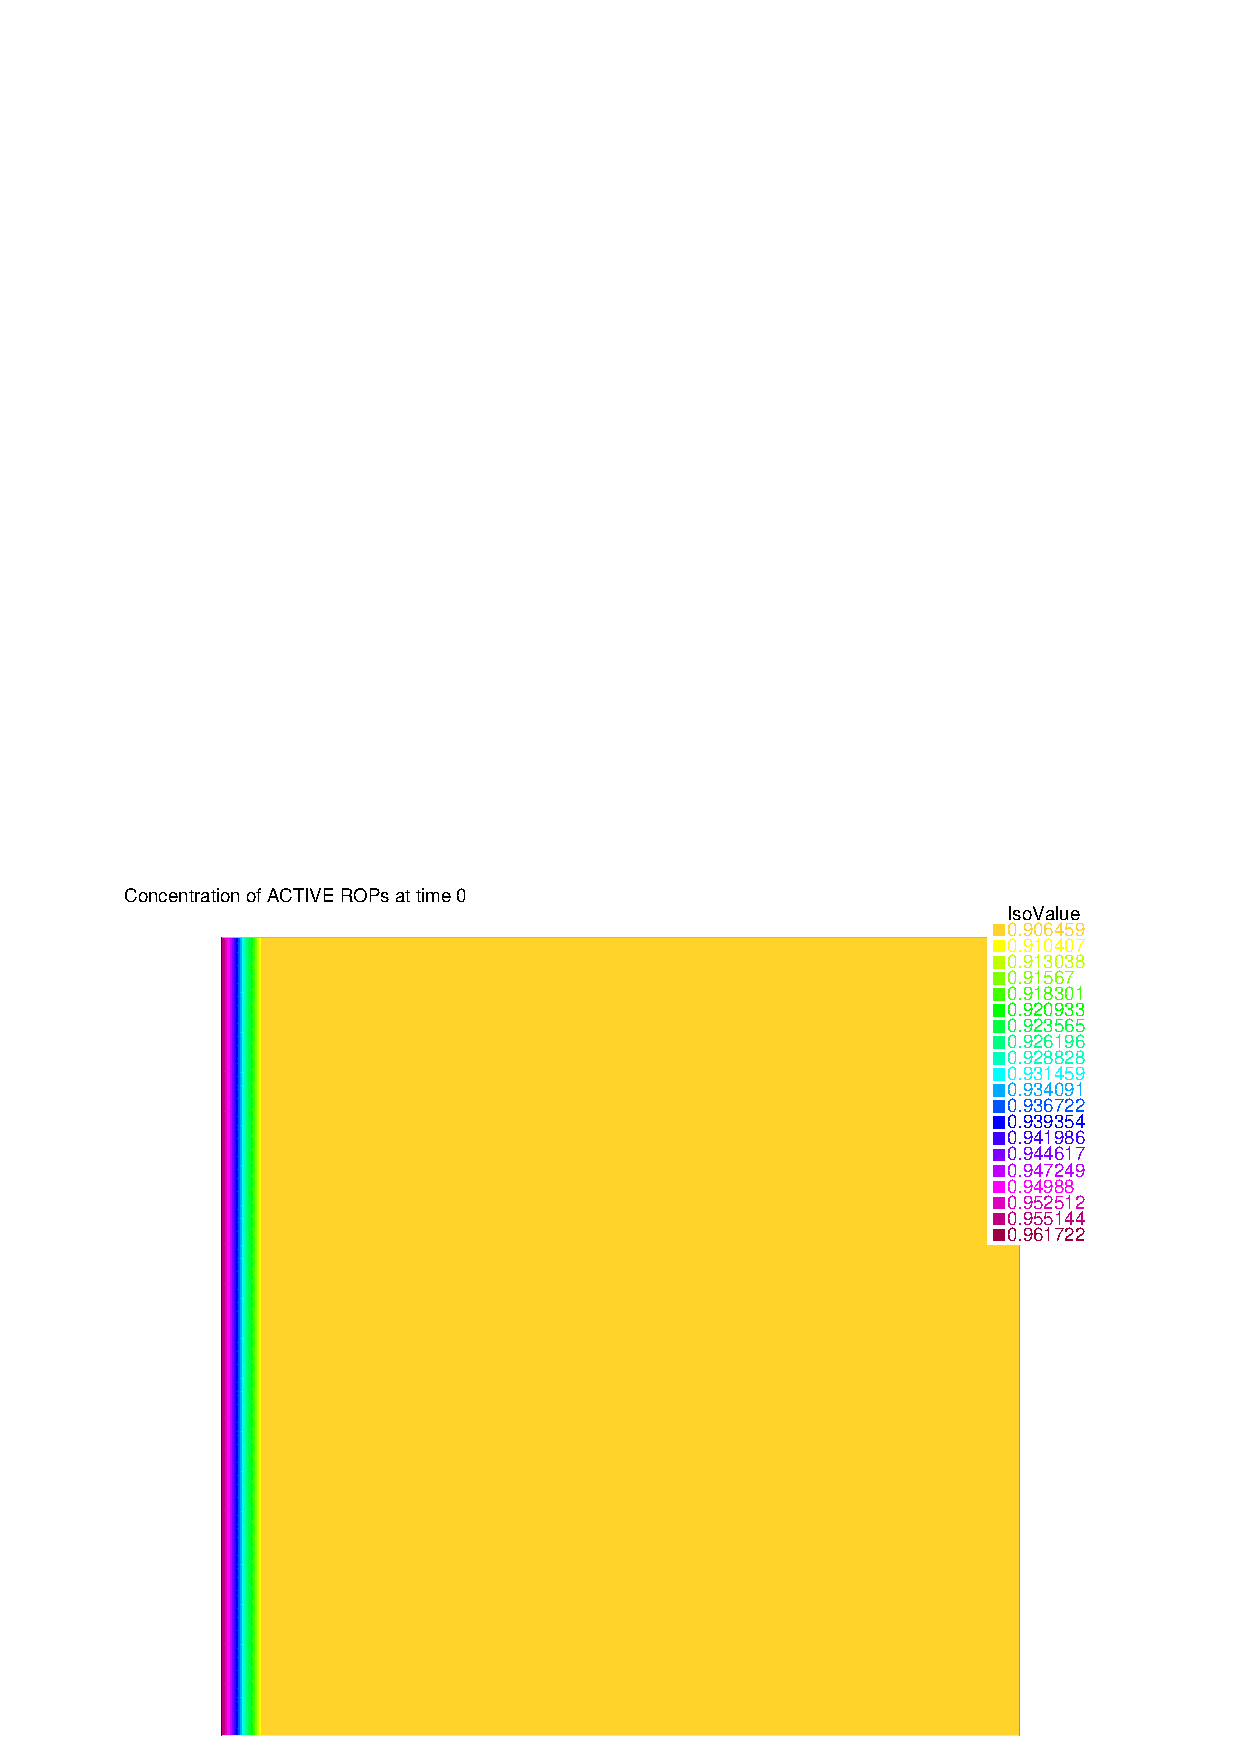
\includegraphics[scale=0.25]{cap2/U0.png}}
    \quad
    \subfloat[Inactive ROPS at iteration $k = 0$.\label{fig:VconstInit}]{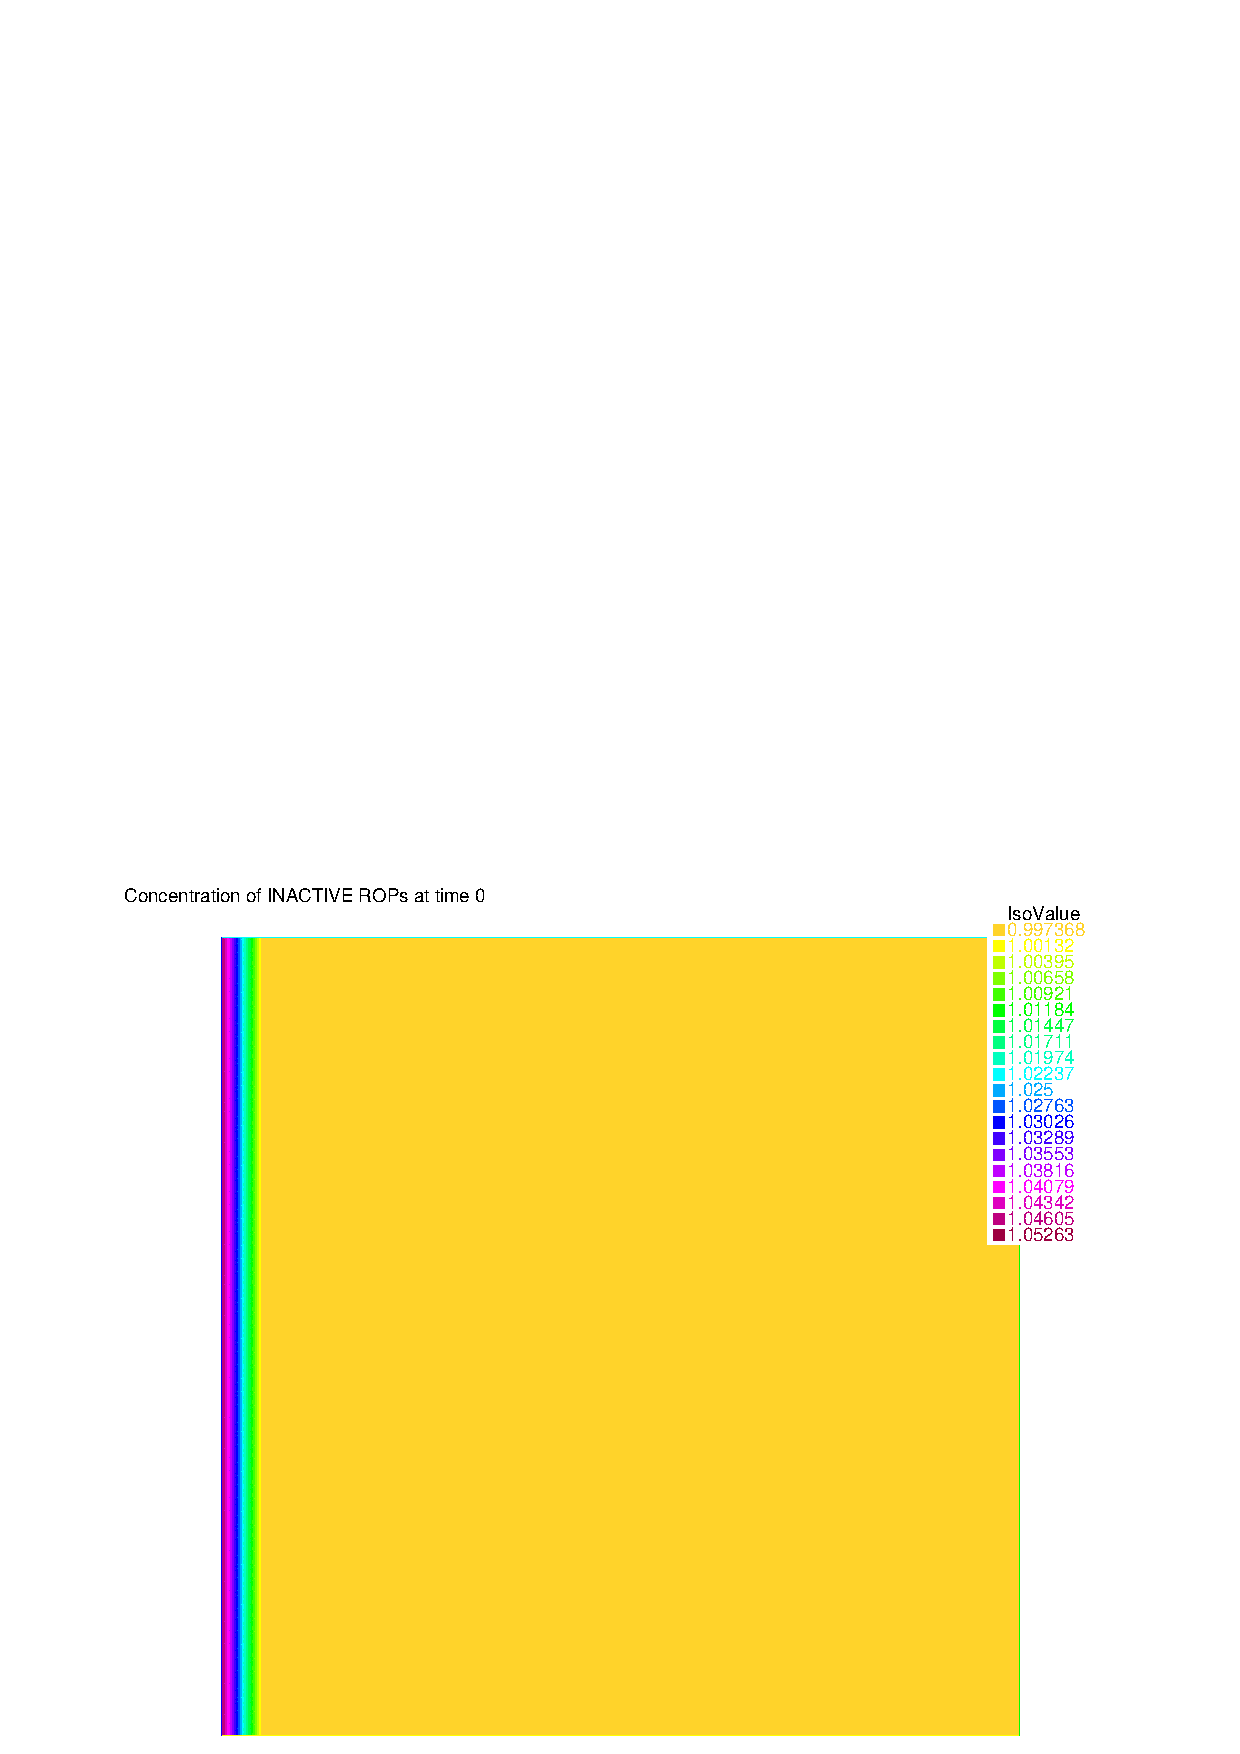
\includegraphics[scale=0.25]{cap2/V0.png}}
    \quad
    \subfloat[Active ROPs at iteration $k = 84$ .\label{fig:Ustationary}]{\includegraphics[scale=0.25]{cap2/statU.png}}
    \quad
    \subfloat[Inactive ROPS at iteration $k = 84$.\label{fig:Vstationary}]{\includegraphics[scale=0.25]{cap2/statV.png}}
    \caption[Equilibrium for Set C]{Solutions of the non homogeneous stationary problem system obtained at convergence.}
    \label{fig:stationarySol}
    % \caption[Stationary system initialization]{Constant homogeneous initialization for stationary problem system.}
    % \label{fig:constInit}
\end{figure}
Under different distribution of auxin, the system converges to another equilibrium, different from the cited one in \cite{intra2} and validated in Section \ref{sec:ValidationNewton}; in order to obtain the new steady state, it has been used as convergence criterion for Newton's method a tolerance \verb|tol = 1e-12| and \verb|MAXiter = 200|. The stationary system converges to a one spot solution for the active ROP as shown in Figure~ \ref{fig:Ustationary}-\ref{fig:Vstationary}, stopping at iteration \verb|k = 84| and reaching a residual of \verb|4.76187e-13|. The obtained solution is the equilibrium of the ROPs system under the whole settings.

% \begin{figure}[H]
%     \centering
%     \subfloat[Active ROPs at iteration $k = 84$ .\label{fig:Ustationary}]{\includegraphics[scale=0.23]{cap2/statU.png}}
%     \quad
%     \subfloat[Inactive ROPS at iteration $k = 84$.\label{fig:Vstationary}]{\includegraphics[scale=0.23]{cap2/statV.png}}
%     \caption[Equilibrium for Set C]{Solutions of the stationary problem system obtained at convergence.}
%     \label{fig:stationarySol}
% \end{figure}
We want to validate the semi-implicit method: we start from the perturbed equilibrium in Figures \ref{fig:Ustationary}-\ref{fig:Vstationary} and we verify that the system converges back to it. The initial state of concentrations $\left[\mathbf{U}^{0}, \mathbf{V}^{0} \right]$ was obtained perturbing the equilibrium with a periodic function of space, modulated with a coefficient $\bar{\epsilon}$ as follows:
\begin{equation} \label{eq:pert}\begin{aligned}
  U & = u^0 + \bar{\epsilon} \ \cos(2\pi\frac{x}{L_x}) \ \cos(2\pi\frac{y}{L_y}) \\
  V & = v^0 + \bar{\epsilon} \ \cos(2\pi\frac{x}{L_x}) \ \cos(2\pi\frac{y}{L_y})
\end{aligned} \end{equation}
We report then the solution of the 1 cell solver with final time $T_{max} = 200s$, obtained with the same set C of parameters.
\begin{figure}
  \centering
  \includegraphics[scale = 0.15]{cap1/max.png}
  \caption{Maximum of active concentration ROPs over time}
  \label{fig:max}
\end{figure}
We plot over time the maximum value of the active concentration of ROPs obtained varying initialization characterized by $\bar{\epsilon} = 10^{-p}$ with $p$ going from 3 to 0. For each of this initial states, the semi-implicit solver implemented converges back to the equilibrium as can be recovered from Figure \ref{fig:max}.

We compare the four solutions obtained at $t = 200s$ with the equilibrium found in the stationary problem. We give as estimate of the error the $L^{\infty}\left(\Omega\right)$ norm of the difference between each final solutions obtained and the stationary one, normalized with the $L^{\infty}\left(\Omega\right)$ norm of the equilibrium solution. The computed errors are reported in Table \ref{tab:error_conv}.

\begin{table}
    % \caption*{Order of convergence w.r.t time}
    \centering
    \begin{tabular}{|p{12em}|c c c c|}
    \hline
     & \textbf{$\bar{\epsilon} = 10^{-3}$} & $\bar{\epsilon} = 10^{-2}$ & $\bar{\epsilon} = 10^{-1}$ &  $\bar{\epsilon} = 10^{-0}$ \T\B\\
    \hline \hline
    $\mathbf{||\bar{U}-U_{h}||_{L^{\infty}\left(\Omega\right)}} / \ \mathbf{||\bar{U}||_{L^{\infty}\left(\Omega\right)}}$ & 4.59967e-07 & 1.9993e-04 & 1.99633e-03 & 2.05963e-02 \T\B\\
    $\mathbf{||\bar{V}-V_{h}||_{L^{\infty}\left(\Omega\right)}} / \ \mathbf{||\bar{V}||_{L^{\infty}\left(\Omega\right)}}$ & 8.23218e-08 & 3.57118e-05 & 3.56417e-4 & 3.65996e-3 \T\B\\
    \hline
    \end{tabular}
    \\[10pt]
    \caption{Errors computed with normalized $L^{\infty}\left(\Omega\right)$ norm of the difference between equilibrium of the system and the converged solution at $t = 200s$.}
    \label{tab:error_conv}
\end{table}

\subsection{Single cell solver convergence analysis}\label{sec:conv}
% -> analisi convergenze ... terrei solo quella L2 tempo e L1 spazio, con integrazione metood trapezio
In this section we present the procedure we used to recover the order of convergence of our method with respect to time interval refinement $\Delta t$. Since the semi-implicit method we applied to solve the RD system under spatial dependent coefficients, we tried to find out empirically the order of convergence of our method.

The system is sensitive to parameters settings and initialization, therefore we decided to take as exact solution of our system the equilibrium under perturbation obtained as in Section \ref{sec:ValidationSS_nothom}, increasing the mesh refinement. More precisely, we solve the stationary system under non-homogeneous auxin distribution $k_{20} \alpha(x) = k_{20} e^{-\nu \frac{x}{L_x}}$ with set C of parameters (Table \ref{tab:setprm}) and refining mesh using \verb|N_x = 800| intervals on $x$ side and \verb|N_y = 240| intervals on y side. Newton's method reaches convergence in 80 iterations; we then solve the time dependent problem using as initial state the stationary solution obtained at iteration 80 perturbed with the periodic function in \eqref{eq:pert}, with $\tilde{\epsilon} = 1$. We solve the system reducing the time-step length up to $\Delta t = 0.001$ and save results for every instant solved up to time $T_{max} = 5.0 s$. The finite element solution obtained with high mesh refinement and small time discretization is taken as reference solution for our analysis:
\begin{equation*}
  \left( u_{ex}, v_{ex} \right) = \left(U_{h,ex}(t), V_{h,ex}(t)\right)
\end{equation*}

In order to inspect the order of convergence with respect to time we run the code for semi-implicit solver for many different values of $\Delta t$. We introduce a loop over possible values of $\Delta t \in  DT = [\Delta t_0,\Delta t_1 ...]$ and we compute the errors of the obtained solution at each time step with respect to the exact solution using different norms. We detail each norm and corresponding formula of approximation:

\textbf{$L^{\infty}$ norm over time of the $L^2$ norm in space}
\begin{equation}\begin{aligned}
  ||U-u_{ex}||_{L^{\infty}\left(0, T; L^2\left(\Omega\right) \right)} & = \sup_{t \in (0, T)} ||U_h(t)-U_{h,ex}(t)||_{L^2\left(\Omega\right)} \\ & \simeq \max_{n = 0, .., M} ||U_h^n - U_{h,ex}^n||_{L^2(\Omega)} \\
  ||V-v_{ex}||_{L^{\infty}\left(0, T; L^2\left(\Omega\right) \right)} & = \sup_{t \in (0, T)} ||V_h(t)-V_{h,ex}(t)||_{L^2\left(\Omega\right)}  \\ & \simeq \max_{n = 0, .., M} ||V_h^n - V_{h,ex}^n||_{L^2(\Omega)}
\end{aligned} \end{equation}

\textbf{ $L^2$ norm over time of the $L^1$ norm in space}
\begin{equation}\label{eq:norm2}\begin{aligned}
  ||U-u_{ex}||_{L^2\left(0, T; L^1\left(\Omega\right) \right)} & = \sqrt{\int_0^{T} \left( ||U_h(t)-U_{h,ex}(t)||_{L^1\left(\Omega\right)} \right)^2 dt} \\ & \simeq \sqrt{ \frac{\Delta t}{2} ||U_h^M- U_{h,ex}^M||_{L^1\left(\Omega\right)}^2 + \Delta t \sum_{n = 1}^{M-1} ||U_h^n - U_{h, ex}^n||_{L^1\left(\Omega\right)}^2 } \\
  ||V-v_{ex}||_{L^2\left(0, T; L^1\left(\Omega\right) \right)} & = \sqrt {\int_0^{T} \left(||V_h(t)-V_{h,ex}(t)||_{L^1\left(\Omega\right)}\right)^2 dt }\\ & \simeq \sqrt{ \frac{\Delta t}{2} \left( ||V_h^M- V_{h,ex}^M||_{L^1\left(\Omega\right)}^2 \right) + \Delta t \sum_{n = 1}^{M-1} ||V_h^n - V_{h, ex}^n||_{L^1\left(\Omega\right)}^2} \\
\end{aligned} \end{equation}

\textbf{$L^2$ norm over time of the $H^1$ norm in space}
\begin{equation}\label{eq:norm3}\begin{aligned}
  ||U-u_{ex}||_{L^2\left(0, T; H^1\left(\Omega\right) \right)} & = \sqrt{\int_0^{T} \left( ||U_h(t)-U_{h,ex}(t)||_{H^1\left(\Omega\right)} \right)^2 dt} \\ & \simeq \sqrt{ \frac{\Delta t}{2} ||U_h^M- U_{h,ex}^M||_{H^1\left(\Omega\right)}^2 + \Delta t \sum_{n = 1}^{M-1} ||U_h^n - U_{h, ex}^n||_{H^1\left(\Omega\right)}^2 } \\
  ||V-v_{ex}||_{L^2\left(0, T; H^1\left(\Omega\right) \right)} & = \sqrt {\int_0^{T} \left(||V_h(t)-V_{h,ex}(t)||_{H^1\left(\Omega\right)}\right)^2 dt }\\ & \simeq \sqrt{ \frac{\Delta t}{2} \left( ||V_h^M- V_{h,ex}^M||_{H^1\left(\Omega\right)}^2 \right) + \Delta t \sum_{n = 1}^{M-1} ||V_h^n - V_{h, ex}^n||_{H^1\left(\Omega\right)}^2}
\end{aligned} \end{equation}
Norms in \eqref{eq:norm2} - \eqref{eq:norm3} are approximated with composite trapezoidal formula \cite{NM:Quarteroni}.

% \begin{equation}\begin{aligned}
%   ||U-u_{ex}||_{L^{\infty}\left(0, T; L^2\left(\Omega\right) \right)} & = \sup_{t \in (0, T)} ||U_h(t)-U_{h,ex}(t)||_{L^2\left(\Omega\right)} \\ & \simeq \max_{n = 0, .., M} ||U_h^n - U_{h,ex}^n||_{L^2(\Omega)} \\
%   ||V-v_{ex}||_{L^{\infty}\left(0, T; L^2\left(\Omega\right) \right)} & = \sup_{t \in (0, T)} ||V_h(t)-V_{h,ex}(t)||_{L^2\left(\Omega\right)}  \\ & \simeq \max_{n = 0, .., M} ||V_h^n - V_{h,ex}^n||_{L^2(\Omega)} \\
%   ||U-u_{ex}||_{L^2\left(0, T; L^1\left(\Omega\right) \right)} & = \sqrt{\int_0^{T} \left( ||U_h(t)-U_{h,ex}(t)||_{L^1\left(\Omega\right)} \right)^2 dt} \\ & \simeq \sqrt{ \frac{\Delta t}{2} ||U_h^M- U_{h,ex}^M||_{L^1\left(\Omega\right)}^2 + \Delta t \sum_{n = 1}^{M-1} ||U_h^n - U_{h, ex}^n||_{L^1\left(\Omega\right)}^2 } \\
%   ||V-v_{ex}||_{L^2\left(0, T; L^1\left(\Omega\right) \right)} & = \sqrt {\int_0^{T} \left(||V_h(t)-V_{h,ex}(t)||_{L^1\left(\Omega\right)}\right)^2 dt }\\ & \simeq \sqrt{ \frac{\Delta t}{2} \left( ||V_h^M- V_{h,ex}^M||_{L^1\left(\Omega\right)}^2 \right) + \Delta t \sum_{n = 1}^{M-1} ||V_h^n - V_{h, ex}^n||_{L^1\left(\Omega\right)}^2} \\
%   ||U-u_{ex}||_{L^2\left(0, T; H^1\left(\Omega\right) \right)} & = \sqrt{\int_0^{T} \left( ||U_h(t)-U_{h,ex}(t)||_{H^1\left(\Omega\right)} \right)^2 dt} \\ & \simeq \sqrt{ \frac{\Delta t}{2} ||U_h^M- U_{h,ex}^M||_{H^1\left(\Omega\right)}^2 + \Delta t \sum_{n = 1}^{M-1} ||U_h^n - U_{h, ex}^n||_{H^1\left(\Omega\right)}^2 } \\
%   ||V-v_{ex}||_{L^2\left(0, T; H^1\left(\Omega\right) \right)} & = \sqrt {\int_0^{T} \left(||V_h(t)-V_{h,ex}(t)||_{H^1\left(\Omega\right)}\right)^2 dt }\\ & \simeq \sqrt{ \frac{\Delta t}{2} \left( ||V_h^M- V_{h,ex}^M||_{H^1\left(\Omega\right)}^2 \right) + \Delta t \sum_{n = 1}^{M-1} ||V_h^n - V_{h, ex}^n||_{H^1\left(\Omega\right)}^2} \\
% \end{aligned}\end{equation}

 The order of convergence is then is estimated by the following formula:
\begin{equation}\label{eq:order_est}
    \alpha \simeq \frac{log(err(\Delta t_i) / err(\Delta t_{i+1}))}{log(\Delta t_i/\Delta t_{i+1})} =: \alpha_{i,i+1}
\end{equation}
where $err(\Delta t_i)$ has to be replaced with the different kind of errors computed with $\Delta t = \Delta t _i$. This estimation gets more exact for decreasing values of time-step length, i.e., for $\Delta t \rightarrow 0$.

Defining the order estimation $ \alpha_{i,i+1}$ as in formula \eqref{eq:order_est}, Table \ref{tab:res_conv} reports the results that we obtain with $\Delta t \in [0.2, 0.125, 0.1, 0.05, 0.025, 0.01, 0.005]$:
\begin{table}
    % \caption*{Order of convergence w.r.t time}
    \centering
    \begin{tabular}{|p{12em}|c c c c c c|}
    \hline
     & \textbf{$\alpha_{0,1}$} & $\alpha_{1,2}$ & $\alpha_{2,3}$ &  $\alpha_{3,4}$ & $\alpha_{4,5}$ & $\alpha_{5,6}$ \T\B\\
    \hline \hline
    $\mathbf{||U-U_{h,ex}||_{L^{\infty}\left(0, T_{max}; L^2\left(\Omega\right) \right)}}$ & 0.3182 & 0.4998 & 0.7059 & 0.8312 & 0.9596 & 1.1123 \T\B\\
    $\mathbf{||V-V_{h,ex}||_{L^{\infty}\left(0, T_{max}; L^2\left(\Omega\right) \right)} }$ & 0.7238 & 0.9478 & 0.8810 & 0.9632 & 1.0410 & 1.1565 \T\B\\
    \hline
    $\mathbf{||U-U_{h,ex}||_{L^2\left(0, T_{max}; L^1\left(\Omega\right) \right)}}$ & 0.8701 &0.8892  & 0.9626 & 1.0009 & 1.0447 & 1.1586 \T\B\\
    $\mathbf{||V-V_{h,ex}||_{L^2\left(0, T_{max}; L^1\left(\Omega\right) \right)}}$ & 0.8569 & 0.89552 & 0.93304 & 0.98439 & 1.0483 &1.1598 \T\B\\
    \hline
    $\mathbf{||U-U_{h,ex}||_{L^2\left(0, T_{max}; H^1\left(\Omega\right) \right)}}$ & 1.2061 & 1.3733 & 1.5646 & 1.7873 &1.9971 & 2.2678 \T\B\\
    $\mathbf{||V-V_{h,ex}||_{L^2\left(0, T_{max}; H^1\left(\Omega\right) \right)}}$ & 1.7200 & 1.7851 & 1.8585 & 1.9582 & 2.0884 & 2.3142 \T\B\\
    \hline
    \end{tabular}
    \\[10pt]
    \caption{Results of estimated order of convergence with respect to time refinement.}
    \label{tab:res_conv}
\end{table}

The order computed with error in the $L^2\left(0, T, H^1 \left(\Omega\right)\right)$ norm is bigger than the other. From the results obtained we can infer that our semi-implicit method has an order of convergence to the exact solution with respect to $\Delta t$ of at least 1 for all norms considered. We then can assume that we have a order of convergence comparable to explicit Euler method. On the other hand, we can expect improved numerical stability properties due to the semi-implicit treatment.
A fully implicit method is expected to have a second order of convergence, but it would require to solve a nonlinear problem at every time-step, resulting in a large computational cost. Overall, we can deem our semi-implicit method a good compromise between the robustness of a fully implicit scheme and the efficiency of an explicit one.

\subsection{Simulation of a single cells system}
In this section we present one result obtained applying the one cell solver method to solve \eqref{eq:LinSys}, imposing Set C of parameters of Table \ref{tab:setprm}, therefore solving the original RD system \eqref{eq:FM} through the semi-implicit method described in Section \ref{sec:SI method}. The initial active and inactive ROPs distribution was settled constant homogeneous:
\begin{equation*}
    \mathbf{U}^0 = 0.9, \ \ \ \mathbf{V}^0 = 1.0
\end{equation*}
as shown in Figure \ref{fig:1cellSolI}.

\begin{figure}[H]
    \centering
    \subfloat[Active ROPs at time $t = 0s$ .\label{fig:U0}]{\includegraphics[scale=0.15]{cap2/2021-11-29_11-37-42/frame.0000.png}}
    \quad
    \subfloat[Inactive ROPS at time $t =180s$.\label{fig:V0}]{\includegraphics[scale=0.15]{cap2/2021-11-29_11-37-42/Vframe.0000.png}}
    \caption[Single cell at $t = 0s$]{Constant homogeneous initialization for 1cell solver.}
    \label{fig:1cellSolI}
\end{figure}

\begin{figure}[H]
    \centering
    \subfloat[Active ROPs at time $t = 3000s$ .\label{fig:U3000}]{\includegraphics[scale=0.15]{cap2/2021-11-29_11-37-42/frame.0499.png}}
    \quad
    \subfloat[Inactive ROPS at time $t = 3000s$.\label{fig:V3000}]{\includegraphics[scale=0.15]{cap2/2021-11-29_11-37-42/Vframe.0499.png}}
    \caption[Single cell at $t = 3000s$]{Solutions of the 1cell solver at final time $t = 3000s$.}
    \label{fig:1cellSolF}
\end{figure}

The dynamical system for the spots was simulated up to final time $T_{max} = 3000s$, and in Figure \ref{fig:1cellSolF} we show the solutions $\mathbf{U}$ and $\mathbf{V}$ obtained. Focusing the attention on the concentration of active ROPs in Figure \ref{fig:1cellUevolution}, its evolution in time and space shows a typical patch formation. From the relevant snapshots, we see the formation of a homoclinic stripe along the left boundary, than it rapidly divides into spots and the system evolves to a steady-state composed by two spots.
% aligned with the direction of the auxin gradient in realtà no ... da vedere
% 2021-11-29_11-37-42
\begin{figure}[H]
    \centering
    \subfloat[U($t = 0s)$ \label{fig:U0t}]{\includegraphics[scale=0.15]{cap2/2021-11-29_11-37-42/frame.0000.png}}
    \quad
    \subfloat[U($t = 54s$) \label{fig:U50}]{\includegraphics[scale=0.15]{cap2/2021-11-29_11-37-42/frame.0009.png}}
    \quad
    \subfloat[U($t = 198s$) \label{fig:U200}]{\includegraphics[scale=0.15]{cap2/2021-11-29_11-37-42/frame.0033.png}}
    \quad
    \subfloat[U($t = 228s$) \label{fig:V225}]{\includegraphics[scale=0.15]{cap2/2021-11-29_11-37-42/frame.0038.png}}
    \quad
    \subfloat[U($t = 258s$) \label{fig:U250}]{\includegraphics[scale=0.15]{cap2/2021-11-29_11-37-42/frame.0043.png}}
    \quad
    \subfloat[U($t = 360s$) \label{fig:U350}]{\includegraphics[scale=0.15]{cap2/2021-11-29_11-37-42/frame.0060.png}}
    \caption[1cell Active ROPs]{Active ROPs $u$ evolution for 1cell solver.}
    \label{fig:1cellUevolution}
\end{figure}
